\scanpage{19}
\mspage{5}

% top left
\figure{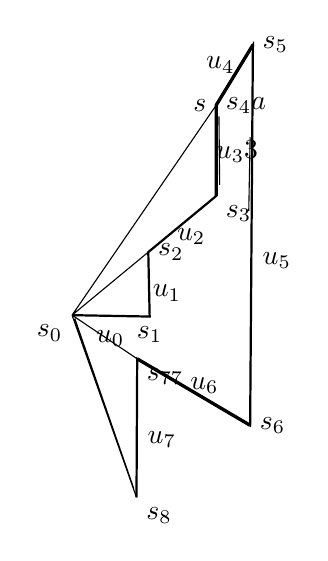
\begin{tikzpicture}[scale=.88]
\coordinate (a) at (0,0); \coordinate (b) at (1.12,-.02); \coordinate (c) at (1.1,.91);
\coordinate (d) at (2.08,1.72); \coordinate (e) at (2.08,3.03); \coordinate (f) at (2.61,3.9);
\coordinate (g) at (2.57,-1.59); \coordinate (h) at (.94,-.63); \coordinate (i) at (.93,-2.63);
\draw[thin] (a)--(c) (a)--(e) (a)--(h) (a)--(i) (.04,-.05)--(.89,-2.5);
\draw[thick] (a)--(b)--(c)--(d)--(e)--(f)--(g)--(h)--(i);
\draw[very thick] (d)--(e)--(f) (g)--(h); \draw (2.13,1.88)--(2.12,2.87) (2.55,1.5)--(2.57,2.57);
\node[below left] at (a) {$s_0$}; \node[below] at (b) {$s_1$}; \node[right] at (c) {$s_2$};
\node[below right] at (d) {$s_3$}; \node[right] at (e) {$s_{4}\unsure{a}$}; \node[left] at (e) {$s$};
\node[right] at (f) {$s_5$}; \node[right] at (g) {$s_6$}; \node[below right] at (h) {$s_{\deleted{\unsure{7}}7}$}; \node[below right] at (i) {$s_8$};
\node at (.55,-.34) {$u_0$}; \node at (1.37,.32) {$u_1$}; \node at (1.72,1.14) {$u_2$};
\node at (2.38,2.36) {$u_{3}\unsure{3}$}; \node at (2.14,3.61) {$u_4$}; \node[right] at (2.61,.79) {$u_5$};
\node at (1.91,-1.02) {$u_6$}; \node[right] at (.95,-1.8) {$u_7$};
\end{tikzpicture}}

% top right
\[
\boxed{\lambda_0=0}\Rightarrow u_1u_{0i}=\lambda_i u_{i-1}u_i
\]

% upper half, coordinate list
\[
\begin{aligned}
s_0&=(0,0)\\
s_1&=(1,0)\\
s_2&=(1,1) &&(y_2=1)\\
s_3&=(\beta_1,\beta_1) &&\beta_1\ne1,0\\
s_4&=(\beta_1,y_4) &&y_4\ne\beta_1\\
s_5&=(\beta_2\beta_1,\beta_2y_4) &&\beta_2\ne1,0\\
s_6&=(\beta_2\beta_1,y_6) &&y_6\ne\beta_2y_4\\
s_7&=(\beta_3\beta_2\beta_1,\beta_3y_6) &&\beta_3\ne1,0\\
s_8&=(\beta_3\beta_2\beta_1,y_8) &&y_8\ne\beta_3y_6\\
{}[\,s_9&=s_0\,] &&[\,\beta_4=0\,]
\end{aligned}
\]

% below coordinate list on right
\[
\begin{gathered}
\deleted{\beta_1\beta_2\mathbin{--}\beta_{\unsure{k|3|8}}}\\
\beta_1\quad\beta_2\quad\beta_3\\
y_4\quad y_6\quad y_8
\end{gathered}
\]

% below horizontal divider
\noindent\rule{\linewidth}{.3pt}

Aucun des $\lambda_i$ nuls \deleted{$\Leftrightarrow$ \unsure{les|ples} $s_i$ tous distincts}

% lower third, general relation
\[
\lambda_i u_{i-1}-\lambda_{i+1}u_i-\lambda_{i+1}u_{i+1}+\lambda_{i+2}u_{i+2}=0
\]

% lower third, four lines on left, three on right
\[
\begin{aligned}
\lambda_1u_0-\lambda_2u_1-\lambda_2u_2+\lambda_3u_3&=0
&\lambda_3u_3&=-\lambda_1u_0+\lambda_2u_1+\lambda_2u_2\\
\lambda_2u_1-\lambda_3u_2-\lambda_3u_3+\lambda_4u_4&=0
&\lambda_4u_4&=-\lambda_1u_0\unsure{+}\qquad(\lambda_2+\lambda_3)u_2\\
&&&\hspace{8em}\deleted{\lambda_3}\\
\lambda_3u_2\deleted{\unsure{+}}-\lambda_4u_3-\lambda_4u_4+\lambda_5u_5&=0
&\lambda_3\lambda_5u_5&=\\
\lambda_4u_3-\lambda_5u_4-\lambda_5u_5+\lambda_6u_6&&&
\end{aligned}
\]

% below recurrences, two long lines
\[
\begin{aligned}
\lambda_3\lambda_5u_5&=\lambda_3[-\lambda_1u_0+(\lambda_2+\lambda_3)u_2]
+\lambda_4(-\lambda_1u_0+\lambda_2u_1+\lambda_2u_2)-\lambda_3^2u_2\\
&=(-\lambda_1(\lambda_3+\lambda_4)u_0+\lambda_2\lambda_4u_1+
\lambda_2(\lambda_3+\lambda_4)u_2\qquad -\, -\, -
\end{aligned}
\]

% bottom left
\[
\deleted{\unsure{x_2|u_2}=\frac{1}{\unsure{\vphantom{1}\smash{-}}}}
\]

% bottom right
\[
u_0\quad u_1\qquad 4
\]

% archive sheet number: 25
